\newpage
%**************************************************************
\chapter{The White Dog s.r.l.}
\label{cap:thewhitedog}

\section{Chi è The White Dog s.r.l.}

The White Dog s.r.l. è una realtà aziendale nata nel 2008 con sede a Torreglia, in provincia di Padova. Essa è stata fondata dal signor Stefano Mocellini, fondatore e CEO di Diana Corp.\footnote[1]{\url{http://www.dianacorp.com/}} , con la volontà di creare un \textit{team} di lavoro focalizzato sulla ricerca e sviluppo. \\
The White Dog s.r.l. coordina e gestisce società tutte affini al settore \textit{e-commerce}, come Diana Corp. e LiveStory\footnote[2]{\url{http://www.livestory.nyc/}}. L'azienda possiede un reparto di ricerca e sviluppo denominato R\&D, il quale esplora nuove tecnologie da applicare poi alle società figlie nel caso di esito positivo o facendo nascere nuovi progetti separati.

\label{The White Dog s.r.l.}
\begin{figure}[ht]
	\begin{center}
		
\includegraphics[scale=1]{twd_logo}
		\caption{Logo dell'azienda The White Dog s.r.l.}
	\end{center}
\end{figure}
\FloatBarrier

\section{Prodotti e servizi}

Il principale servizio che l'azienda offre alle aziende che coordina e gestisce, come Diana Corp. e Live Story, è la ricerca e lo sviluppo di nuove tecnologie da applicare nell'ambito del \textit{fashion e-commerce}. Essa svolge l'attività di \textit{testing} delle nuove tecnologie web disponibili, le valuta attentamente in termini di prestazioni e costi, per poi renderle disponibili. Ad essa oltretutto vengono commissionati progetti che Diana Corp., per competenze e tempistiche, non può portare a termine, come ad esempio applicazioni \textit{mobile} legate agli \textit{e-commerce} prodotti. \\ \\
The White Dog s.r.l. inoltre ha creato il \textit{concept} di \textit{Live Story}, \textit{social management system}\ped{\hyperlink{sms}{G}} che gestisce contenuti \textit{social} e li rende acquistabili, \textit{concept} che è diventato azienda a se stante nel 2015 con sede a New York. \textit{Live Story} colleziona foto degli utenti dei \textit{social network} marcate con un particolare \textit{hashtag} che rappresenta l'azienda che vuole utilizzare il servizio. Il sistema accoppia la foto ad un particolare prodotto presente nel catalogo e genera automaticamente le richieste di permesso di utilizzo della foto e la invia all'utente interessato. Se l'utente approva e il moderatore ritiene conforme la foto, l'azienda può utilizzare il contenuto nel proprio sito/\textit{e-commerce}.

\section{Processi interni}

Lo sviluppo del software a The White Dog s.r.l. segue una metodologia tipicamente Agile\footnote[3]{\url{http://agilemanifesto.org/}}. Questa metodologia permette all'azienda di rispondere in tempi brevi ai continui nuovi bisogni di Diana Corp. e Live Story, anche loro fortemente legate a questo metodo di lavoro. Essendo The White Dog s.r.l. formata da un \textit{team} composto da poche persone, tale metodo di lavoro risulta essere molto efficiente.

\label{Metodologia Agile}
\begin{figure}[ht]
	\begin{center}
		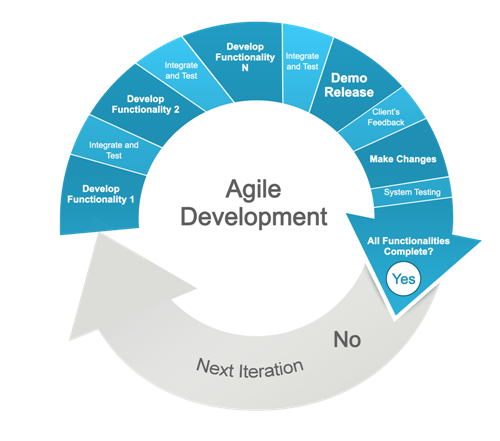
\includegraphics[height=8cm]{agile_development}
		\caption{Metodologia di sviluppo Agile}
	\end{center}
\end{figure}
\FloatBarrier

Le procedure, gli strumenti e le metriche adottate in The White Dog s.r.l. derivano da tre principali concetti di sviluppo Agile:

\subsubsection{DevOps}

Metodologia di sviluppo software che punta alla comunicazione, collaborazione e integrazione tra gli sviluppatori e addetti alle \textit{operations}\ped{\hyperlink{ops}{G}} dell'\textit{information technology}. DevOps vuole rispondere all'interdipendenza tra sviluppo software e IT \textit{operations}\ped{\hyperlink{ops}{G}}, puntando ad aiutare un'organizzazione a sviluppare in modo più rapido ed efficiente prodotti e servizi.

\label{DevOps}
\begin{figure}[ht]
	\begin{center}
		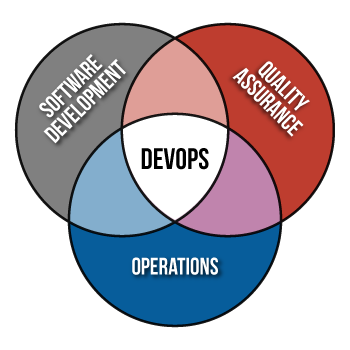
\includegraphics[scale=0.5]{devops-diagram}
		\caption{Competenze necessarie alla metodologia di sviluppo DevOps}
	\end{center}
\end{figure}
\FloatBarrier

In The White Dog s.r.l. questo principio è concretizzato dal fatto che ogni membro possiede sia le competenze di sviluppo, sia amministrative che di controllo della qualità, migliorando così di molto l'efficienza e l'agilità nello sviluppo del software e nel suo rilascio.

\subsubsection{Extreme Programming}

Metodologia di sviluppo software che enfatizza la scrittura di codice di qualità e la rapidità di risposta ai cambiamenti di requisiti. Prescrive lo sviluppo iterativo e incrementale, soprattutto in brevi cicli di sviluppo. Suggerisce inoltre l'uso sistematico di \textit{unit testing}\ped{\hyperlink{ut}{G}} e \textit{refactoring}\ped{\hyperlink{ref}{G}}, vietando ai programmatori di sviluppare codice non strettamente necessario. Sostiene la chiarezza e la semplicità del codice, preferisce strutture gestionali non gerarchiche e dà molta importanza  alla comunicazione diretta e frequente fra sviluppatori e cliente e fra gli sviluppatori stessi. 

\label{Extreme Programming}
\begin{figure}[ht]
	\begin{center}
		
\includegraphics[scale=0.11]{extremeprogramming}
		\caption{Metodologia di sviluppo software Extreme Programming}
	\end{center}
\end{figure}
\FloatBarrier

Il \textit{team} di sviluppo di The White Dog s.r.l. fa ampio utilizzo di questa metodologia, spingendo molto sulla semplicità del codice prodotto, che dovrà poi essere utilizzato dagli sviluppatori Diana Corp. e Live Story, e sulla giornaliera comunicazione diretta tra gli sviluppatori e con il loro principali clienti. Questa comunicazione è facilitata dal fatto che The White Dog s.r.l. ha sede nello stesso stabilimento di Diana Corp..

\subsubsection{Scrum}

\textit{Framework} agile di sviluppo software, iterativo ed incrementale, concepito per gestire progetti e prodotti software. Esso enfatizza tutti gli aspetti di gestione di progetto legati a contesti in cui è difficile pianificare in anticipo. Vengono utilizzati meccanismi propri di un processo di controllo empirico, in cui i cicli di \textit{feedback} che ne costituiscono le tecniche di \textit{management} fondamentali risultano in opposizione alla gestione basata sul concetto tradizionale di \textit{command-and-control}\ped{\hyperlink{cac}{G}}. Il suo approccio alla pianificazione e gestione dei progetti è quello di portare l'autorità decisionale al livello di proprietà e certezze operative.

\label{Scrum board}
\begin{figure}[ht]
	\begin{center}
		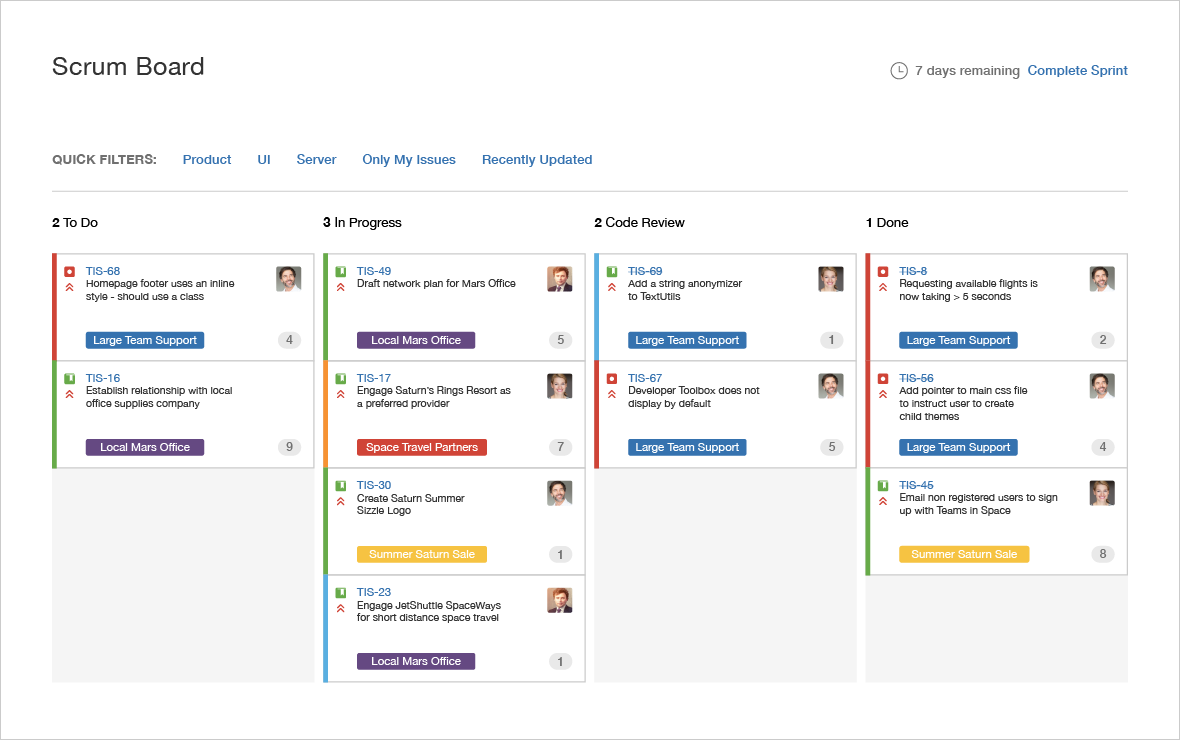
\includegraphics[scale=0.35]{scrumboard}
		\caption{Esempio di \textit{scrum board} all'interno del software Jira}
	\end{center}
\end{figure}
\FloatBarrier

The White Dog s.r.l. sfrutta questa metodologia di sviluppo software utilizzando ampiamente strumenti di \textit{project management} che supportano il metodo Scrum come Wrike e Jira.

\section{Strumenti e tecnologie}

\subsection{Ambienti di sviluppo}

Il sistema operativo adottato dall'azienda è Mac OS X installato su macchine iMac. \\
L'ambiente di sviluppo, data la natura aziendale, non è standardizzato, ma varia in base al prodotto in fase di sviluppo, che può cambiare in maniera repentina. 

\subsection{Gestione dei progetti}

I due principali strumenti utilizzati da The White Dog s.r.l. per il \textit{project management} e l'\textit{issue tracking}\ped{\hyperlink{it}{G}} sono rispettivamente Wrike\footnote[4]{\url{https://www.wrike.com/it/it/}} e Jira\footnote[5]{\url{https://www.atlassian.com/software/jira}}.\\
Wrike, sviluppato dall'omonima casa, è uno strumento \textit{online} per la collaborazione e il \textit{project management}. Permette ai suoi utenti di modificare progetti, classificare le attività per importanza, tenere traccia dei programmi e collaborare con altri utenti dello stesso gruppo.\\
Jira prodotto dall'azienda Atlassian è un software di \textit{bug tracking}\ped{\hyperlink{bg}{G}}, \textit{issue tracking}\ped{\hyperlink{it}{G}} e \textit{project management}. Esso permette di tenere traccia delle azioni e dei problemi degli utenti, di distribuire i compiti all'interno del \textit{team}, discutere del lavoro in atto con una visibilità completa e migliorare le prestazioni della squadra visualizzando dati in tempo reale.

\subsection{Versionamento}

Il principale software di controllo di versione distribuito utilizzato dall'azienda è Git\footnote[6]{\url{https://git-scm.com/}}. Git supporta lo sviluppo non lineare con diramazione e fusioni rapide e continue e comprende strumenti specifici per visualizzare e navigare una cronologia di sviluppo non lineare. Permette ad ogni sviluppatore una copia locale dell'intera cronologia di sviluppo e le modifiche vengono importate da un \textit{repository}\ped{\hyperlink{rep}{G}} ad un altro. I \textit{repository}\ped{\hyperlink{rep}{G}} possono essere pubblicati facilmente tramite protocolli HTTP, FTP, SSH, RSYNC o uno speciale protocollo git.

\subsection{Tecnologie di sviluppo}

Vista la varietà delle ricerche e dei prodotti sviluppati dall'azienda The White Dog s.r.l., le tecnologie di sviluppo sono sempre in continua evoluzione e cambiamento. Le principali sono comunque Java, JavaScript, Node.js, MongoDB, PHP, HTML, CSS e AWS.

\section{Ricerca e innovazione}

R\&D rappresenta il reparto di ricerca e sviluppo dell'azienda The White Dog s.r.l..
Ha a disposizione diversi dispositivi per la ricerca come \textit{smartphone} di ultima generazione, \textit{Smart TV}, \textit{smartwatch} e numerosi dispositivi per lo sviluppo \textit{AR}\ped{\hyperlink{ar}{G}} e \textit{VR}\ped{\hyperlink{vr}{G}} come \textit{Google Glass}, \textit{Oculus Rift Development Kit 2}, \textit{Google Cardboard} e \textit{Leap Motion}. Attraverso questi dispositivi l'azienda studia e sviluppa nuove modalità di interazione che l'utente finale può utilizzare nell'acquisto nei propri \textit{stores} digitali.
